%\documentclass[english,twoside]{article}
\documentclass[english,twoside]{labmanual} 
%labmanual.cls is a modified version of article.cls, tweaked to handle \part{} differently

%% LyX 1.1 created some parts of this file.  For more info, see http://www.lyx.org/.
%% Do not edit unless you really know what you are doing.

\usepackage[T1]{fontenc}
\usepackage[nomarginpar]{geometry}
\usepackage{tocloft} %Allow us to leave page numbers for Parts out of table of contents
\cftpagenumbersoff{part} %No page numbers for Parts out of table of contents
\renewcommand{\cftsecdotsep}{\cftsubsecdotsep}
%\usepackage{newclude} %Allows use of /include*{}
%DANGER DANGER: newclude is NOT compatible with package xr, used for external references.
\geometry{verbose,letterpaper}
\usepackage{fancyhdr}
\usepackage{babel}
\setlength\parskip{\medskipamount}
\setlength\parindent{0pt}
\usepackage{graphicx}
\usepackage{wrapfig}
%\usepackage{epstopdf} %this package apparently allows pdflatex to work on this document, since all we use are eps figures.
\usepackage{comment}
\usepackage{esvect}
\usepackage{amsmath} %uncommented by MT 5/2015, used in "E near charged rod"
\usepackage{mathtools} %added by MT 6/2015, for access to dcases environment in finding_v_from_e
\usepackage{tabularx} %added by MT 6/2015, for fixed width columns, used in rc_circuits
\usepackage{microtype}
\usepackage{titlesec}
\usepackage{xr}

%For fixed width columns:
\newcolumntype{L}[1]{>{\raggedright\arraybackslash}p{#1}}
\newcolumntype{C}[1]{>{\centering\arraybackslash}p{#1}}
\newcolumntype{R}[1]{>{\raggedleft\arraybackslash}p{#1}}


\addtolength{\oddsidemargin}{1.0cm} %without these two lines, larger margin is on the OUTSIDE.  We want the larger edge on the INSIDE, to allow room for the three hole punches
\addtolength{\evensidemargin}{-1.0cm}

\setlength\topmargin{0.2in}
\addtolength{\hoffset}{-1.0cm}
\addtolength{\textwidth}{2.0cm}
\addtolength{\voffset}{-1.5cm} %This line is apparently needed on some versions of MikTex XeLatex.  Comment out if your pages appear shifted too high.
\addtolength{\textheight}{3.5cm}
% define a strut for extra vertical space in tables.
\newcommand{\hi}{\rule[-2mm]{0mm}{6mm}}

\pagestyle{fancy}
%\fancyhead[LE,RO]{\slshape \rightmark} %This is the default for fancy page style
%\fancyhead[LO,RE]{\slshape \leftmark}
\fancyhead[LO,RE]{\slshape \rightmark} 
\fancyhead[LE,RO]{\slshape \leftmark} % Reversed LE, RO to  LO,RE to make headers come out correctly on even/odd pages



%%%%%%%%%%%%%%%%%%%%%%%%%%%%%% LyX specific LaTeX commands.
\providecommand{\LyX}{L\kern-.1667em\lower.25em\hbox{Y}\kern-.125emX\@}
\newenvironment{LyXParagraphIndent}[1]%
{
  \begin{list}{}{%
    \setlength\topsep{0pt}%
    \addtolength{\leftmargin}{#1}
    \setlength\parsep{0pt plus 1pt}%
  }
  \item[]
}
{\end{list}}
%% Special footnote code from the package 'stblftnt.sty'
%% Author: Robin Fairbairns -- Last revised Dec 13 1996
\makeatletter
\let\SF@@footnote\footnote
\def\footnote{\ifx\protect\@typeset@protect
    \expandafter\SF@@footnote
  \else
    \expandafter\SF@gobble@opt
  \fi
}
\expandafter\def\csname SF@gobble@opt \endcsname{\@ifnextchar[%]
  \SF@gobble@twobracket
  \@gobble
}
\edef\SF@gobble@opt{\noexpand\protect
  \expandafter\noexpand\csname SF@gobble@opt \endcsname}
\def\SF@gobble@twobracket[#1]#2{}
\makeatother


%I make use of some latex features to manage the section numbers. To use those you have to insert the following lines into the latex preamble (before the %"\begin{document}" command).

% two new commands to do labelling. - gpg 12/4/13
\newcommand{\customlabel}[2]{%
\protected@write \@auxout {}{\string \newlabel {#1}{{#2}{}}}}

\newcommand{\actlabel}[1]{%
\protected@write \@auxout {}{\string \newlabel {#1}{{\arabic{activity}}{}}}}

\newcommand{\makelabheader}
%{Name: \rule{2.0in}{0.1pt}\hfill{}Section: \rule{1.0in}{0.1pt}\hfill{}Date: \rule{1.0in}{0.1pt}}
{Name: \rule{2.0in}{0.1pt}\hfill{}Lab Partner(s): \rule{3.0in}{0.1pt}}

%\newcommand{\dir131}{../../131/StudentGuideModule1} %This does not work, because commands can only be made of numeric characters, not numbers.

%A new command for putting a box around a paragraph:
\newenvironment{newboxed} %maybe there's a better way to do this.  I just cribbed from the web. --MT
    {\begin{center}
    \begin{tabular}{|p{0.9\textwidth}|}
    \hline\\
    }
    { 
    \\\\\hline
    \end{tabular} 
    \end{center}
    }

\newcounter{activity}

%  The following command, \answerspace, should be used to replace \vspace.
%  \vspace{} is not ideal for an answer space for students, for two reasons:
%  1. It can be ignored if it comes at the end of a page, and
%  2. The spacing is exact, and Latex will not stretch or compress it at all to make things fit on a page, which means
%  that other things WILL get stretched or compressed to make things fit, which means those other things will 
%  end up looking bad, and leading to a lot of underfull \vbox warnings.
%  \answerspace fixes both of those problems, specifically allowing the space to grow to up to twice the stated size.
\newcommand{\answerspace}[1]{\vspace*{#1 plus #1}}

%  The next several lines implement \includelab, which replaces \include.
%  Usage is \includelab{1}{file} to include it, or \includelab{0}{file} to NOT include it.  
%  But all 0's can be overridden by writing \includealllabstrue in the master.tex file, which is easier than deleting 
%  fifty individual `%' signs and then remembering to put them all back, which is what you had to do before.
%  \includeonly still works as you expect it to.
\newif\ifincludealllabs
\newcommand{\includelab}[2]{
	\ifnum#1=1
		\include{#2}
	\else {
		\ifincludealllabs
		 	\include{#2}
		\fi}
	\fi
}
 %all general latex packages, commands, and definitions now here.

%The \includeonly line below is a great way to save time so you don't always have to compile the WHOLE latex document, if for instance you've only made changes to a single lab.  If you want to compile more than two labs, the syntax is \includeonly{lab1,lab2,lab3} with no spaces after the commas.
%The master.pdf produced will have only the title page, TOC, and that single lab, though the other lab names will appear in the TOC.
%\includeonly{standing_waves_strings/standing_waves_strings}

%Use the following line to override all of the 1's and 0's in the \includelab statements below
%\includealllabstrue

%\renewcommand{\section}{\cleardoublepage\NoExtraPageSection} %Makes each lab start on odd numbered page (right hand side).

\makeindex
\begin{document}

\newgeometry{total={8in,10.5in},hoffset=0.2in,voffset=0.6in}
%nb: I just messed with the numbers above until it looked okay.  I really don't know what I'm doing. --MT, 4/23/2016
\thispagestyle{empty}
\definecolor{darkblue}{RGB}{0,0,160}
\definecolor{lighterblue}{RGB}{0,128,255} %This one looks better on the printshop's printer
\newpagecolor{lighterblue}

\begin{center}
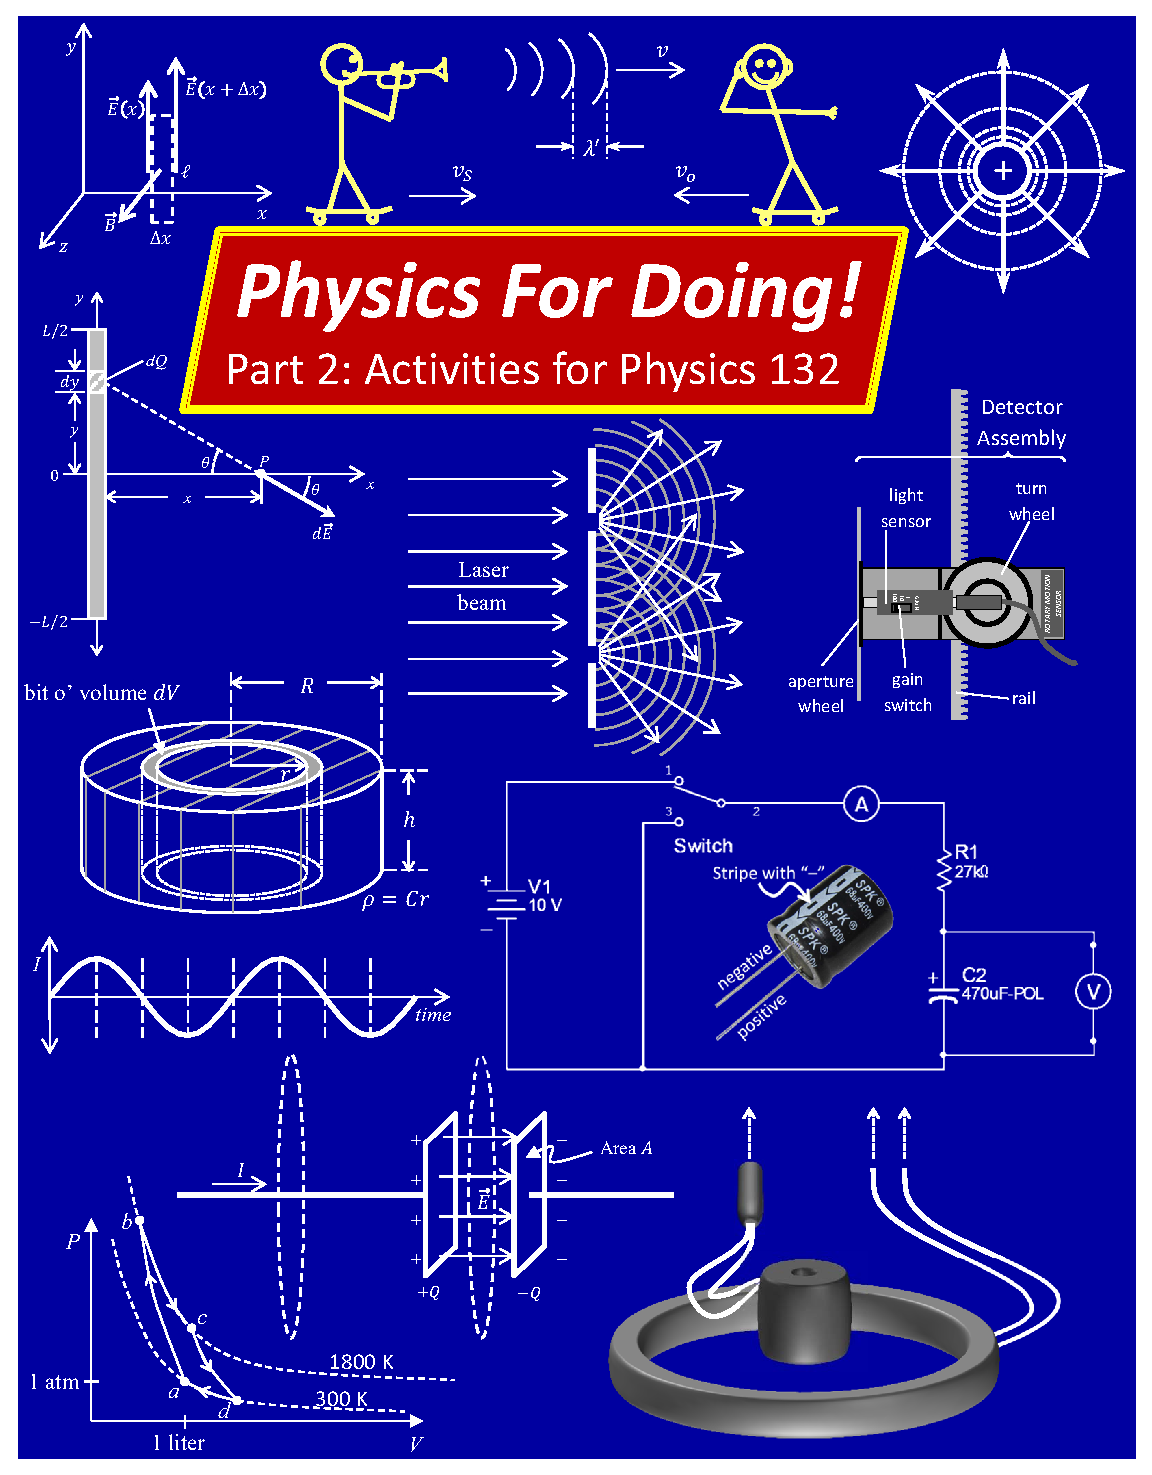
\includegraphics[width=7.3in,trim={0 0 .1cm 0},clip]{132_front_pages/132_front_cover.eps}
\index{color page}
\end{center}
\newpage

\restoregeometry
\restorepagecolor
\thispagestyle{empty}

\
\vfill
\textit{Cover art: Various graphics and diagrams from the activities in this manual.  Yep, you'll be doing stuff.}
\pagebreak


\title{Physics For Doing!\\
Part 2: Activities for Physics 132}

\author{Matthew G. Belk}
\author{Emory F. Bunn}
\author{Mirela Fetea\footnote{Current address: Germanna Community College, Fredericksburg, VA}}
\author{Gerard P. Gilfoyle}
\author{Henry Nebel}
\author{Philip D. Rubin\footnote{Current address: Department of Physics, George Mason University, Fairfax, VA}}
\author{Jack Singal}
\author{Matthew L. Trawick}
\author{Michael F. Vineyard\footnote{Current address: Department of Physics, Union College, Schenectady, NY}}
\affil{Department of Physics, University of Richmond, VA}


\maketitle

\vspace{0.8in}

%\begin{abstract}

\begin{center}
\large{\textbf{Welcome to Physics 132!}}
\end{center}

The exercises in this manual have been developed to support an investigative
physics course that emphasizes active learning. 
%The units are made up of activities designed to guide your investigations in the laboratory. 
Your written work will consist primarily of documenting
your class activities by filling in the entries in the spaces provided
in the units. The entries consist of observations, derivations, calculations,
and answers to questions. Although you may use the same data and graphs
as your partner(s) and discuss concepts with your classmates, all
entries should reflect your own understanding of the concepts and
the meaning of the data and graphs you are presenting. Thus, each
entry should be written in your own words. It is very important
to your success in this course that your entries reflect a sound understanding
of the phenomena you are observing and analyzing. 

Some of these exercises
have been taken from the Workshop Physics project at Dickinson College
and the Tools for Scientific Thinking project at Tufts University
and modified for use at the University of Richmond. Others have been
developed locally. 
We wish to acknowledge the support we have received for this project
from the University of Richmond and the Instrumentation and Laboratory
Improvement program of the National Science Foundation. 
%\end{abstract}


\newpage
\
\thispagestyle{plain}

\newpage
\
%\setcounter{page}{2} %changed from 1 to 2 on 6/9/15 by MT.  The reason is that in the circuit labs, the odd pages need to be on the right (the fronts of each sheet of paper) and the even pages need to be on the left.  This is critical, because these labs have some pages that are meant to be cut out with scissors, so the backs have to be left blank.  This is done by using the \cleardoublepage command, which requires that the odd/even pages not be reversed from the usual.


\setcounter{tocdepth}{1}\tableofcontents{}

%use \includelab[1] to include, or \includelab[0] to exclude.  Can be overridden with \includealllabstrue
%--------------------------------------------
\part{Mechanical Waves}

\includelab{1}{standing_waves_strings/standing_waves_strings}
\includelab{1}{resonance_tubes}
\includelab{1}{doppler_shift/doppler_shift}
\includelab{0}{piano_tuning/piano_tuning}


%--------------------------------------------
\part{Electrostatics}

\includelab{1}{electroscope/electroscope}
\includelab{1}{charge_density/charge_density}
\includelab{0}{elec_grav/elec_grav}
\includelab{1}{electric_field_near_a_charged_rod/electric_field_near_a_charged_rod}
\includelab{0}{electric_potential/electric_potential}
\includelab{1}{potential_intro/potential_intro}
\includelab{1}{electric_fields_and_equipotential_lines/ef_equipot_lines}
\includelab{0}{elec_potential_example/elec_potential_example}
\includelab{1}{potential_superposition/potential_superposition}
\includelab{1}{potential_charge_distributions/potential_charge_distributions}
\includelab{1}{finding_v_from_e/finding_v_from_e}
\includelab{0}{electric_field_and_electric_potential/EF_EP_1}
\includelab{0}{electric_field_and_electric_potential/EF_EP_2}
\includelab{0}{electric_field_and_electric_potential/EF_EP_3}
\includelab{0}{electric_field_and_electric_potential/EF_EP_4}
\includelab{0}{electric_field_atomic_nucleus/electric_field_atomic_nucleus}
\includelab{0}{charge_dist_water_mol/charge_dist_water_mol}
\includelab{0}{capacitance}

%--------------------------------------------
\part{Electric Circuits}

\includelab{1}{electric_circuits/electric_circuits}
\includelab{1}{electric_circuits2/electric_circuits2}
\includelab{1}{electric_power/electric_power}
\includelab{1}{rc_circuits/rc_circuits}
\includelab{0}{lr_circuit/lr_circuit}
\includelab{0}{lrc_circuit/lrc_circuit}

%--------------------------------------------
\part{Magnetism}

\includelab{0}{magnetism_qualitative}
\includelab{1}{magnetism_field_perm_mag/magnetism_field_perm_mag}
\includelab{1}{magnetism_currents/magnetism_currents} %need to fix Rotate 270 warning for grayscale figure
\includelab{1}{magnetic_field_earth}
\includelab{1}{biot_savart_straight_wire/biot_savart_straight_wire} 
\includelab{1}{biot_savart_above_loops/biot_savart_above_loops} 
\includelab{1}{amperes_law_infinite_sheet/amperes_law_infinite_sheet}
\includelab{1}{eoverm/eoverm} %need to fix Rotate 270 warning for grayscale figure

%--------------------------------------------
\part{Induction and Electromagnetic Waves}

\includelab{1}{induction_intro/induction_intro} %need to fix Rotate 270 warning for grayscale figure
\includelab{1}{induction_sinusoidal/induction_sinusoidal}
\includelab{0}{generator}
\includelab{1}{deriving_em_waves/deriving_em_waves}
\includelab{1}{plane_waves/plane_waves}

%--------------------------------------------
\part{Wave Optics}

\includelab{1}{interference_of_light/interference} %need to fix Rotate 270 warning for grayscale figure
\includelab{1}{diffraction_of_light/diffraction}
\includelab{1}{diffraction_grating}
\includelab{1}{hydrogen} %Currently listed under both quantum and wave optics.  Be sure it's not selected for both!

%--------------------------------------------
%\part{Geometric Optics}

\includelab{0}{refraction_of_light/refraction_of_light}
\includelab{0}{refraction_at_spherical_surfaces}

%--------------------------------------------
\part{Thermodynamics}

\includelab{0}{heat_temp_int_energy/heat_temp_int_energy}
\includelab{1}{calorimetry/calorimetry}
\includelab{1}{boyles_law/boyles_law}
\includelab{0}{charles_law/charles_law}
\includelab{1}{P-T_relationship_of_gas/P-T}
\includelab{1}{kin_theory_ideal/kin_theory_ideal}
\includelab{1}{applying_kinetic_theory/applying_kinetic_theory}
\includelab{1}{latent_heat_of_vaporization_of_nitrogen/heat_vap_nit_minimalist}
\includelab{1}{expansion_constant_pressure/expansion_constant_pressure}
\includelab{1}{ideal_gas_cycles/ideal_gas_cycles}
\includelab{0}{EinsteinSolid/einstein_solid}
\includelab{0}{S+T/entropy_temperature}
\includelab{1}{entropy_is_it_possible/entropy_is_it_possible}

%--------------------------------------------
%\part{Quantum Mechanics}

\includelab{0}{hydrogen} %Currently listed under both quantum and wave optics.  Be sure it's not selected for both!
\includelab{0}{solveSE/solveSE}
\includelab{0}{qmProbability/qmProbability}
\includelab{0}{radiocarbon_dating/radiocarbon_dating}

%--------------------------------------------
%\part{Other Topics}

\includelab{0}{centripetalForceFor132/centripetalForceFor132}
\includelab{0}{cons_ang_momFor132/cons_ang_mom}
\includelab{0}{impulseFor132/impulse}
\includelab{0}{galilean_relativity}
\includelab{0}{twins_paradox}

%--------------------------------------------
%\part{Appendices}
\immediateaddcontentsline{toc}{part}{Appendices} %Avoids a Roman part number for the Appendices in the toc
\cleardoublepage
\renewcommand{\section}{\NoExtraPageSection} %Makes NO extra page break after each appendix; Appendices can start on odd or even page (right or left side).
\appendix

\includelab{1}{appendices/datastudio_from131}
\includelab{0}{appendices/capstone_from131}
\includelab{1}{appendices/treatment_data_from131}
\includelab{1}{appendices/one_page_uncertainty_from131}
\includelab{1}{appendices/excel_from131}
\includelab{0}{appendices/video_analysis_tracker_from131}
\includelab{0}{appendices/nuke_safety/nuke_safety}
\includelab{0}{appendices/instrumentation_from131}
\end{document}
